\begin{frame}
\frametitle{Mean exit time. Setting}
Given a domain $D \subset \R^d$, $f\colon D \to \R^d, g\colon D \to \R^{d \times m}$ and an $m$-dimensional standard Wiener process $W(t)$, consider
\begin{equation*}
\left \{
\begin{aligned}
	dX(t) &= f(X(t)) dt + g(X(t))dW(t), && 0 < t \leq T, \\
	X(0)  &= X_0, && X_0 \in D.
\end{aligned} \right .
\end{equation*}
The equation is defined in a domain $D$ $\rightarrow$ boundary conditions
\begin{itemize}
	\item \textit{killing boundaries}: $X(t)$ is stopped,
	\item \textit{reflecting boundaries}: $X(t)$ is reflected normally inside $D$.
\end{itemize}
\end{frame}

\begin{frame}
\frametitle{Mean exit time. Problem statement}
\underline{Problem}. Estimate the exit time of the trajectories
\begin{equation*}
	\tau = \min\{\tau_e,T\}, \text{ where } \tau_e = \min\{t\colon X(t)\notin D\}.
\end{equation*}
Another quantity of interest, given $F\colon D \to \R$
\begin{equation*}
	\phi = \phi(T,X_0,F) = \mathbbm{1}_{\{T < \tau_e\}}F(X(T)).
\end{equation*}
If $F \equiv 1$, exit probability 
\begin{equation*}
	\Phi(T,X_0) \defeq \Pr(\tau < T | X(0) = X_0) = 1 - \mathbb{E}(\phi(T,X_0,1)). 
\end{equation*}
\underline{Goal}. Estimate numerically $\tau$ and $\phi$.
\end{frame}

\begin{frame}[plain]
\frametitle{Discrete Euler-Maruyama}
Method:
\begin{equation*}
	\left \{
	\begin{aligned}
		X_h^d(t_{i+1}) &= f(X(t_i))h + g(X(t_i))(W(t_{i+1}) - W(t_{i})),  \\
		X_h^d(0) &= X_0.
	\end{aligned} \right .
\end{equation*}
Parameters of interest computed naively
\begin{equation*}
\begin{aligned}
	\tau_h^d &= \min\{\tau_{h,e}^d,T\}, \text{ where } \tau_{h,e}^d = \min \{t_i \colon X_h^d(t_i) \notin D\}, \\
	\phi_h^d &= \mathbbm{1}_{\{T < \tau_{h,e}^d\}}F(X_h^d(T)).
\end{aligned}
\end{equation*}
Missed exits $\Rightarrow$ 1/2 loss in weak order:
\begin{align*}
	|\mathbb{E}(\tau_h^d) - \mathbb{E}(\tau)| &= O(\sqrt{h}), \\
	|\mathbb{E}(\phi_h^d) - \mathbb{E}(\phi)| &= O(\sqrt{h}).
\end{align*}	
\end{frame}

\begin{frame}[plain]
\frametitle{Continuous Euler-Maruyama}
\underline{Goal}. Restore the order of convergence 1 of Euler-Maruyama in $\R^d$ $\Rightarrow$ Brownian bridge approach.

Method:
\begin{equation*}
	\left \{
	\begin{aligned}
		X_h^c(t) &= f(X(t_i))(t-t_i) + g(X(t_i))(W(t) - W(t_{i})),  && t_i < t \leq t_{i+1},\\
		X_h^c(0) &= X_0.
	\end{aligned} \right .
\end{equation*} 
Estimate at each time step the probability of exit. If $D$ is an half-space
\begin{equation*}
\begin{aligned}
	&\Pr (\exists t \in [ t_i,t_{i+1} ] \quad X_h^d(t) \notin D | X_h^d(t_i) = x_i, X_h^d(t_{i+1}) = x_{i+1}) \\
	&\quad = p(x_i,x_{i+1},h) \\
	&\quad = \exp\Big(-2\frac{[n\cdot(x_i - z_i)][n\cdot(x_{i+1} - z_i)]}{hn\cdot (gg^T(x_i)n)}\Big),
\end{aligned}
\end{equation*}
\end{frame}

\begin{frame}
\frametitle{Continuous Euler-Maruyama}
Parameters of interest. Given $u$ a realization of $U$ uniform r.v. in $(0,1)$
\begin{equation*}
\begin{aligned}
	\tau_h^c &= \min \{T,\tau_{h,e}^c\}, \\
	\text{ where } \tau_{h,e}^c &= \min\{\tau_{h,e1}^c, \tau_{h,e2}^c\}, \\
	\tau_{h,e1}^c &= \min\{t_i = hi \colon X_h(t_i) \notin D\}, \\
	\tau_{h,e2}^c &= \min\{t_i = hi \colon u < p(x_{i-1},x_i,h) \}, \\
	\phi_h^c &= \mathbbm{1}_{\{T < \tau_{h,e}^c\}}F(X_h^c(T)).
\end{aligned}
\end{equation*}
Weak order 1 is restored:
\begin{align*}
	|\mathbb{E}(\tau_h^c) - \mathbb{E}(\tau)| &= O(h), \\
	|\mathbb{E}(\phi_h^c) - \mathbb{E}(\phi)| &= O(h).
\end{align*}
\end{frame}

\subsection{A PDE approach}\label{sec:PDEs}
It is possible to express the mean exit time and the probability of exit from a domain in terms of the solution of partial differential equations (PDE's).
Let us denote by $\Gamma_k,\Gamma_r$ the killing and reflecting subsets of $\partial D$. We consider then the expectation of the exit time from the domain $D$ for a trajectory that at $t=0$ is at position $x$, \textit{i.e.},
\begin{equation}\label{eq:ExpTau}
	\bar\tau(x) = \mathbb{E}(\tau | X(0) = x).
\end{equation}
Let us define the operator $\mathcal L$ induced by \eqref{eq:GeneralModel}, which is applied to a function $u\colon \mathbb{R}^d \rightarrow \mathbb{R}$  as follows
\begin{equation}\label{eq:LOperator}
	\mathcal Lu = f \cdot \nabla u + \frac{1}{2} gg^T : \nabla \nabla u,
\end{equation}
where the $:$ operator between two matrices $A,B$ in $\mathbb{R}^{d\times d}$ is defined as follows
\begin{equation}\label{eq:twoPoints}
	A : B = \sum_{i,j = 1}^d \{A\}_{ij}\{B\}_{ij} = \text{tr}(A^TB).
\end{equation}
The following result allows computing the mean exit time as the solution of an appropriate PDE.

\begin{theorem} Let $\mathcal L$ be the differential operator defined as \eqref{eq:LOperator}. Then, if $\Gamma_k$ and $\Gamma_r$ are respectively the killing and reflecting subsets of $\partial D$, such that $\Gamma_k \cup \Gamma_r = \partial D, \Gamma_k \cap \Gamma_r = \emptyset$, the mean exit time $\bar \tau(x)$ for the solution $X(t)$ of \eqref{eq:GeneralModel} with $X_0 = x$ is the solution of the following boundary value problem
\begin{equation}\label{eq:PDETau}
\left \{
\begin{aligned}
	\mathcal L \bar \tau(x) &= -1, && \text{in } D, \\
	\bar\tau(x) &= 0, && \text{on } \Gamma_k, \\
	\nabla \bar\tau(x) \cdot n &= 0, && \text{on } \Gamma_r,
\end{aligned} \right .
\end{equation}
where $n$ is the normal to $\Gamma_r$.
\end{theorem}
\noindent Further analytic treatment of the mean exit time can be found in \cite{Krumscheid2015,Pavliotis2014}. \\
We now consider the probability of exit from $D$ for a solution $X(t)$ that is equal to $x$ for at a time $s$ smaller than the final time $T$. This probability is the solution of a boundary value problem.
\begin{theorem} Let $\mathcal L$ be the differential operator defined as \eqref{eq:LOperator}. Then, if $\Gamma_k$ and $\Gamma_r$ are respectively the killing and reflecting subsets of $\partial D$, such that $\Gamma_k \cup \Gamma_r = \partial D, \Gamma_k \cap \Gamma_r = \emptyset$
\begin{equation}\label{eq:ExitProbNotation}
	\Pr(\tau < T | X(s) = x) = \Phi(x,s,T) 
\end{equation}
where $\Phi(x,t,T)$ is the solution of the following backwards PDE
\begin{equation}\label{eq:PDEPhi}
\left \{
\begin{aligned}
	\frac{\partial}{\partial t} \Phi(x,t,T) + \mathcal L \Phi(x,t,T) &= 0 && \text{in } D, s \leq t < T, \\
	\Phi(x,t,T) &= 1 && \text{on } \Gamma_k, s \leq t \leq T,\\
	\nabla \Phi(x,t,T) \cdot n &= 0, && \text{on } \Gamma_r, s \leq t \leq T, \\
	\Phi(x,T,T) &= 0 && \text{in } D,
\end{aligned} \right .
\end{equation}
where $n$ is the normal to $\Gamma_r$.
\end{theorem}
\noindent The proof in case $\Gamma_k = \partial D$ of this result can be found in \cite{Sirovich2010}. Further treatment in case of mixed boundary conditions and the closed form of the solution for some particular geometries of $D \subset \mathbb{R}^2$ can be found in \cite{Grebenkov2014}. It is therefore possible to approximate the mean exit time and the exit probability by means of classical methods for solving PDE's numerically, such as finite differences or the Finite Elements Method. In Appendix \ref{sec:Appendix1} we present an analytic formula to compute the mean exit time in the one-dimensional case, and in Appendix \ref{sec:Appendix2} we show a finite difference approach to approximate numerically \eqref{eq:PDETau} in the one-dimensional case. In the two-dimensional case, we solve \eqref{eq:PDETau} and \eqref{eq:PDEPhi} using linear Finite Elements using the PDE toolbox of Matlab.


\begin{frame}
\frametitle{One-dimensional case - Setup}
Consider $D=[-1,1]$ and the SDE
\begin{equation*}
\left \{
\begin{aligned}
	dX(t) &= f(X(t)) dt + g(X(t))dW(t), && 0 < t \leq T, \\
	X(0)  &= X_0, && X_0 \in D.
\end{aligned} \right .
\end{equation*}
Set mixed boundary conditions and
\begin{equation*}
\begin{split}
	f(x) &= -V'(x), \text{ where } V(x) = 0.1(8x^4 - 8x^2 + x + 2), \\
	g(x) &= \sigma \in \R.
\end{split}
\end{equation*}
\underline{Goal}. Verify the weak order of convergence of DEM and CEM.
\underline{Reference solution}. Solution of PDE's
\begin{itemize}
	\item Analytic solution in one-dimensional case for $\bar \tau$,
	\item Finite Differences for $\Phi$.
\end{itemize}
\end{frame}

\begin{frame}
\frametitle{One-dimensional case - Results}
\begin{figure}[t]
    \centering
    \begin{subfigure}{0.49\linewidth}
        \centering
        \resizebox{1\linewidth}{!}{% This file was created by matlab2tikz.
%
%The latest updates can be retrieved from
%  http://www.mathworks.com/matlabcentral/fileexchange/22022-matlab2tikz-matlab2tikz
%where you can also make suggestions and rate matlab2tikz.
%
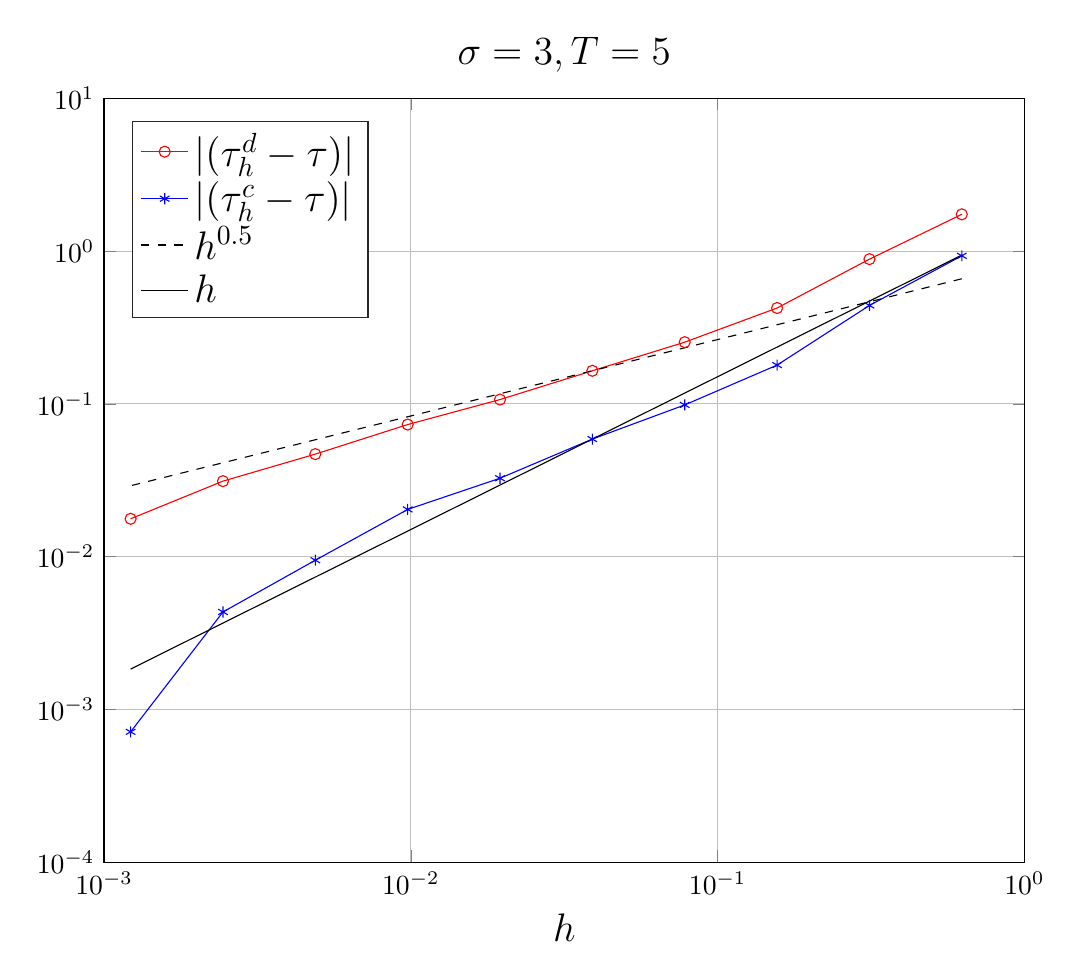
\begin{tikzpicture}

\begin{axis}[%
width=4.602in,
height=3.82in,
at={(0.772in,0.516in)},
scale only axis,
title = {$\sigma = 3, T = 5$},
title style = {font = \Large},
xmode=log,
xmin=0.001,
xmax=1,
xminorticks=false,
xlabel={$h$},
xlabel style={font=\Large},
xmajorgrids,
ymode=log,
ymin=0.0001,
ymax=10,
yminorticks=false,
ymajorgrids,
axis background/.style={fill=white},
legend style={at={(0.03,0.97)},anchor=north west,legend cell align=left,align=left,draw=white!15!black,font=\Large}
]
\addplot [color=red,solid,mark=o,mark options={solid}]
  table[row sep=crcr]{%
0.625	1.73914617431998\\
0.3125	0.885146174319978\\
0.15625	0.423927424319978\\
0.078125	0.253357111819978\\
0.0390625	0.164665705569978\\
0.01953125	0.106693049319978\\
0.009765625	0.0732106274449781\\
0.0048828125	0.0468932446324781\\
0.00244140625	0.0312094067418531\\
0.001220703125	0.0176961010777906\\
};
\addlegendentry{$|\E(\tau_h^d - \tau)|$};

\addplot [color=blue,solid,mark=asterisk,mark options={solid}]
  table[row sep=crcr]{%
0.625	0.931021174319978\\
0.3125	0.440614924319978\\
0.15625	0.179380549319978\\
0.078125	0.098419611819978\\
0.0390625	0.058821955569978\\
0.01953125	0.0326110180699781\\
0.009765625	0.0203737133824781\\
0.0048828125	0.00948064697622808\\
0.00244140625	0.00434612549185309\\
0.001220703125	0.000713688961271941\\
};
\addlegendentry{$|\E(\tau_h^c - \tau)|$};

\addplot [color=black,dashed]
  table[row sep=crcr]{%
0.625	0.658662822279912\\
0.3125	0.465744948149596\\
0.15625	0.329331411139956\\
0.078125	0.232872474074798\\
0.0390625	0.164665705569978\\
0.01953125	0.116436237037399\\
0.009765625	0.082332852784989\\
0.0048828125	0.0582181185186995\\
0.00244140625	0.0411664263924945\\
0.001220703125	0.0291090592593497\\
};
\addlegendentry{$h^{0.5}$};

\addplot [color=black,solid]
  table[row sep=crcr]{%
0.625	0.941151289119649\\
0.3125	0.470575644559824\\
0.15625	0.235287822279912\\
0.078125	0.117643911139956\\
0.0390625	0.058821955569978\\
0.01953125	0.029410977784989\\
0.009765625	0.0147054888924945\\
0.0048828125	0.00735274444624726\\
0.00244140625	0.00367637222312363\\
0.001220703125	0.00183818611156181\\
};
\addlegendentry{$h$};

\end{axis}
\end{tikzpicture}%
 }  
        \caption{Approximation of $\tau$}
        \label{fig:KillOneDPhi}
    \end{subfigure}
    \begin{subfigure}{0.49\linewidth}
        \centering
        \resizebox{1\linewidth}{!}{% This file was created by matlab2tikz.
%
%The latest updates can be retrieved from
%  http://www.mathworks.com/matlabcentral/fileexchange/22022-matlab2tikz-matlab2tikz
%where you can also make suggestions and rate matlab2tikz.
%
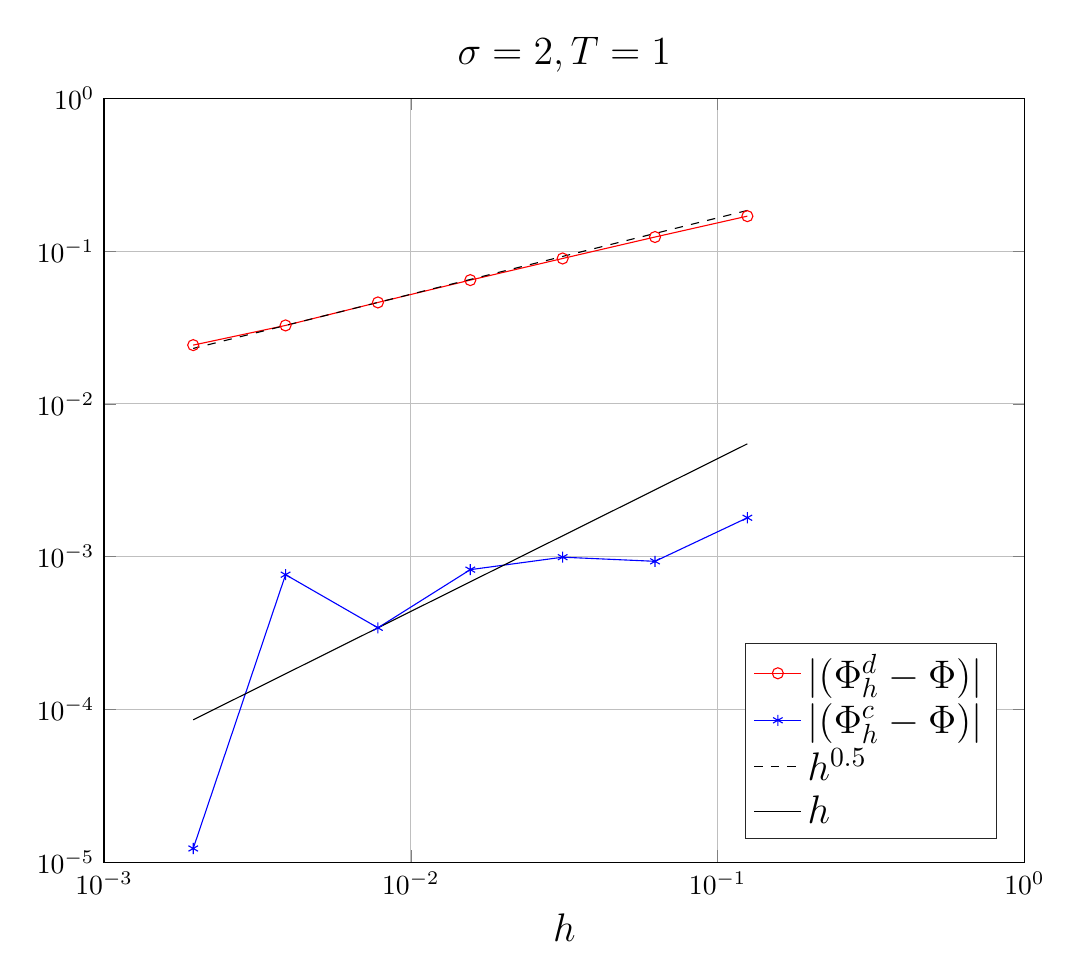
\begin{tikzpicture}

\begin{axis}[%
width=4.602in,
height=3.82in,
at={(0.772in,0.516in)},
scale only axis,
title = {$\sigma = 2, T = 1$},
title style = {font = \Large},
xmode=log,
xmin=0.001,
xmax=1,
xminorticks=false,
xlabel={$h$},
xlabel style = {font=\Large},
xmajorgrids,
ymode=log,
ymin=1e-05,
ymax=1,
yminorticks=false,
ymajorgrids,
axis background/.style={fill=white},
legend pos = south east,
legend style={legend cell align=left,align=left,draw=white!15!black,font=\Large}
]
\addplot [color=red,solid,mark=o,mark options={solid}]
  table[row sep=crcr]{%
0.125	0.169237691826179\\
0.0625	0.123577691826179\\
0.03125	0.0894376918261789\\
0.015625	0.0645576918261789\\
0.0078125	0.0461076918261789\\
0.00390625	0.032607691826179\\
0.001953125	0.024237691826179\\
};
\addlegendentry{$|\E(\Phi_h^d - \Phi)|$};

\addplot [color=blue,solid,mark=asterisk,mark options={solid}]
  table[row sep=crcr]{%
0.125	0.00179769182617895\\
0.0625	0.000932308173821061\\
0.03125	0.000992308173821121\\
0.015625	0.000822308173821118\\
0.0078125	0.000342308173821082\\
0.00390625	0.000762308173821058\\
0.001953125	1.23081738211406e-05\\
};
\addlegendentry{$|\E(\Phi_h^c - \Phi)|$};

\addplot [color=black,dashed]
  table[row sep=crcr]{%
0.125	0.184430767304716\\
0.0625	0.130412246220603\\
0.03125	0.0922153836523578\\
0.015625	0.0652061231103013\\
0.0078125	0.0461076918261789\\
0.00390625	0.0326030615551507\\
0.001953125	0.0230538459130895\\
};
\addlegendentry{$h^{0.5}$};

\addplot [color=black,solid]
  table[row sep=crcr]{%
0.125	0.00547693078113731\\
0.0625	0.00273846539056866\\
0.03125	0.00136923269528433\\
0.015625	0.000684616347642164\\
0.0078125	0.000342308173821082\\
0.00390625	0.000171154086910541\\
0.001953125	8.55770434552705e-05\\
};
\addlegendentry{$h$};

\end{axis}
\end{tikzpicture}%
 }  
        \caption{Approximation of $\Phi$}
        \label{fig:ReflectOneDPhi}
    \end{subfigure}    
    \caption{Results for the one-dimensional case.}
\end{figure}
\end{frame}

\begin{frame}
\frametitle{One-dimensional case - Results}
\begin{figure}[t]
    \centering
    \begin{subfigure}{0.49\linewidth}
        \centering
        \resizebox{1\linewidth}{!}{% This file was created by matlab2tikz.
%
%The latest updates can be retrieved from
%  http://www.mathworks.com/matlabcentral/fileexchange/22022-matlab2tikz-matlab2tikz
%where you can also make suggestions and rate matlab2tikz.
%
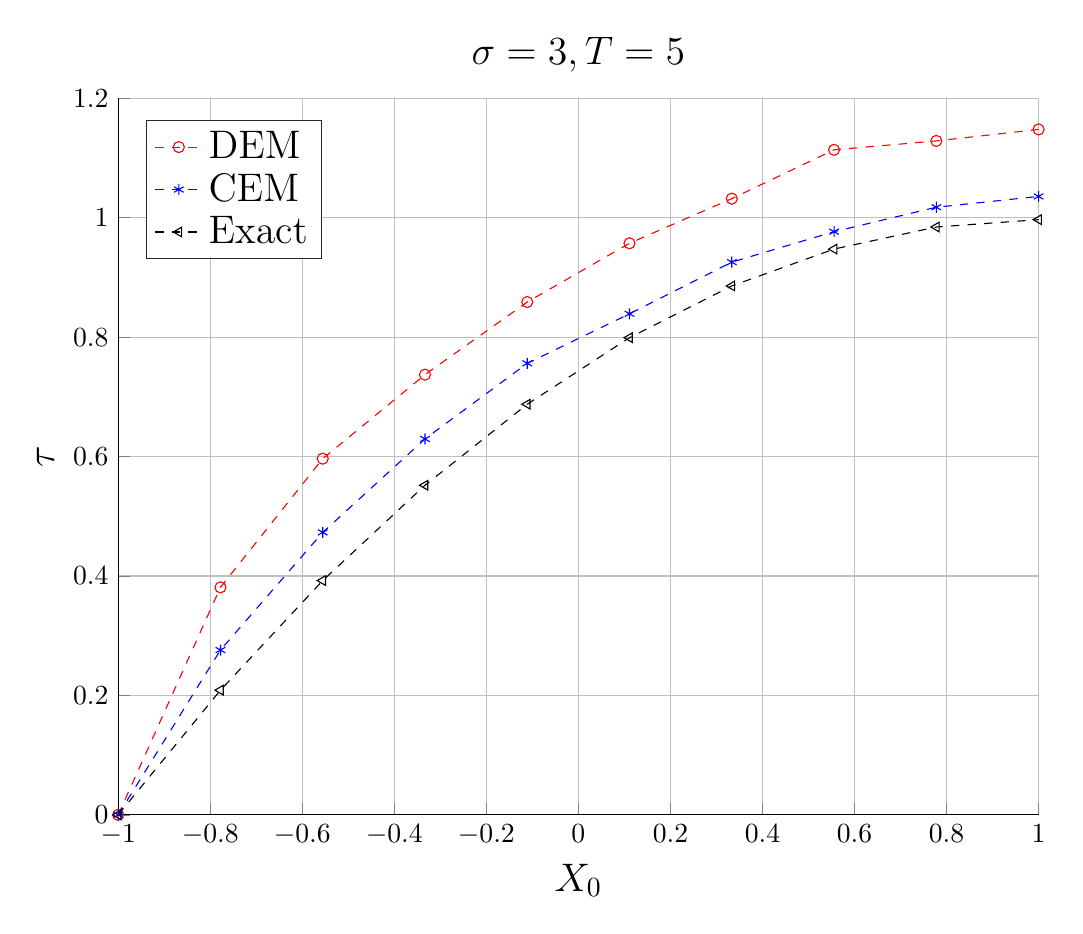
\begin{tikzpicture}

\begin{axis}[%
width=4.602in,
height=3.583in,
at={(0.772in,0.484in)},
scale only axis,
title = {$\sigma = 3, T = 5$},
title style = {font = \Large},
xmin=-1,
xmax=1,
xlabel={$X_0$},
xlabel style={font=\Large},
xmajorgrids,
ymin=0,
ymax=1.2,
ylabel={$\tau$},
ylabel style={font=\Large},
ymajorgrids,
axis background/.style={fill=white},
axis x line*=bottom,
axis y line*=left,
legend pos = north west,
legend style={legend cell align=left,align=left,draw=white!15!black,font=\Large}
]
\addplot [color=red,dashed,mark=o,mark options={solid}]
  table[row sep=crcr]{%
-1	0\\
-0.777777777777778	0.3809765625\\
-0.555555555555556	0.5964609375\\
-0.333333333333333	0.73715625\\
-0.111111111111111	0.8587265625\\
0.111111111111111	0.9571171875\\
0.333333333333333	1.031859375\\
0.555555555555556	1.113609375\\
0.777777777777778	1.1285390625\\
1	1.1478046875\\
};
\addlegendentry{DEM};

\addplot [color=blue,dashed,mark=asterisk,mark options={solid}]
  table[row sep=crcr]{%
-1	0\\
-0.777777777777778	0.275953125\\
-0.555555555555556	0.4729921875\\
-0.333333333333333	0.629484375\\
-0.111111111111111	0.7560703125\\
0.111111111111111	0.8390625\\
0.333333333333333	0.9255703125\\
0.555555555555556	0.976546875\\
0.777777777777778	1.017515625\\
1	1.035609375\\
};
\addlegendentry{CEM};

\addplot [color=black,dashed,mark=triangle,mark options={solid,rotate=90}]
  table[row sep=crcr]{%
-1	0\\
-0.777777777777778	0.208777054487475\\
-0.555555555555556	0.392333503315235\\
-0.333333333333333	0.551939853868488\\
-0.111111111111111	0.687661056545228\\
0.111111111111111	0.79906851214989\\
0.333333333333333	0.885727939207175\\
0.555555555555556	0.947463001823471\\
0.777777777777778	0.984384604394486\\
1	0.996687130893952\\
};
\addlegendentry{Exact};

\end{axis}
\end{tikzpicture}%
 }  
        \caption{Approximation of $\tau$}
        \label{fig:KillOneDPhi}
    \end{subfigure}
    \begin{subfigure}{0.49\linewidth}
        \centering
        \resizebox{1\linewidth}{!}{% This file was created by matlab2tikz.
%
%The latest updates can be retrieved from
%  http://www.mathworks.com/matlabcentral/fileexchange/22022-matlab2tikz-matlab2tikz
%where you can also make suggestions and rate matlab2tikz.
%
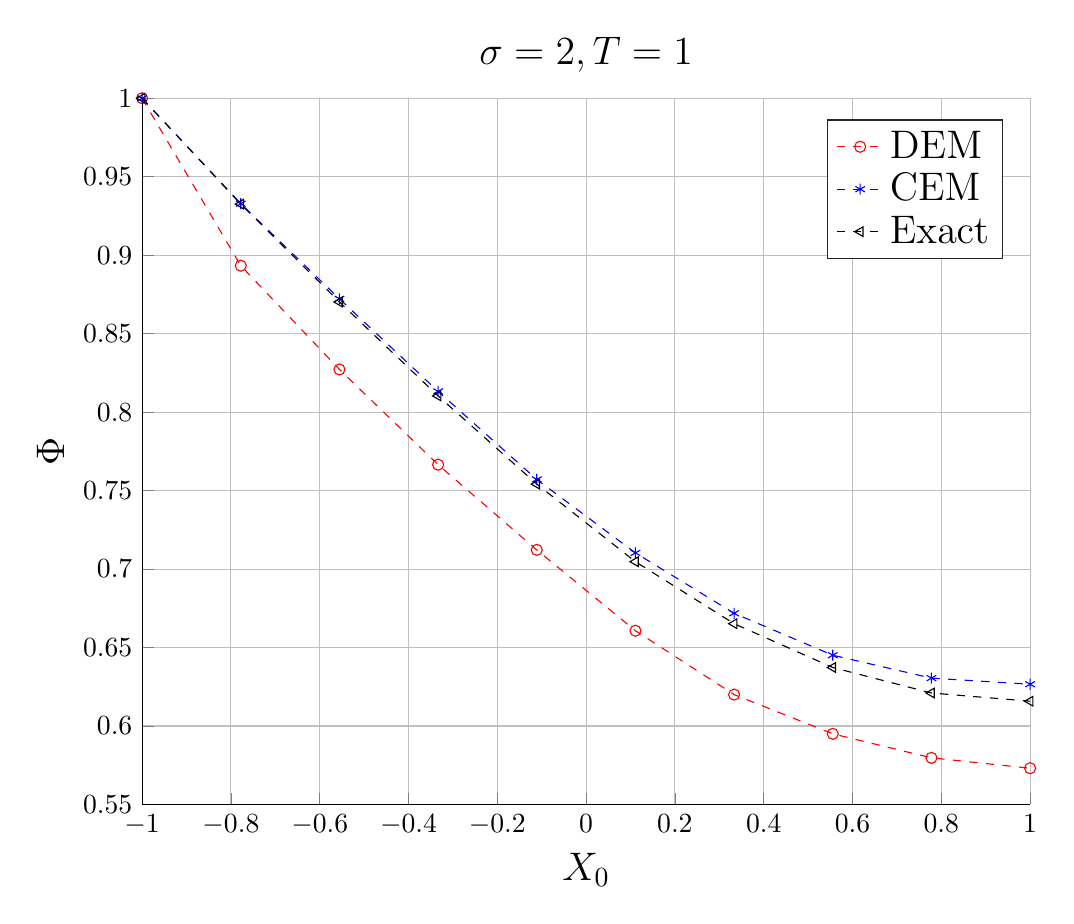
\begin{tikzpicture}

\begin{axis}[%
width=4.44in,
height=3.531in,
at={(0.745in,0.496in)},
scale only axis,
title = {$\sigma = 2, T = 1$},
title style = {font = \Large},
xmin=-1,
xmax=1,
xlabel={$X_0$},
xlabel style={font=\Large},
xmajorgrids,
ymin=0.55,
ymax=1,
ylabel={$\Phi$},
ylabel style={font=\Large},
ymajorgrids,
axis background/.style={fill=white},
axis x line*=bottom,
axis y line*=left,
legend pos = north east,
legend style={legend cell align=left,align=left,draw=white!15!black,font = \Large}
]
\addplot [color=red,dashed,mark=o,mark options={solid}]
  table[row sep=crcr]{%
-1	1\\
-0.777777777777778	0.8933\\
-0.555555555555556	0.8272\\
-0.333333333333333	0.7665\\
-0.111111111111111	0.7122\\
0.111111111111111	0.6607\\
0.333333333333333	0.62\\
0.555555555555556	0.595\\
0.777777777777778	0.5797\\
1	0.5731\\
};
\addlegendentry{DEM};

\addplot [color=blue,dashed,mark=asterisk,mark options={solid}]
  table[row sep=crcr]{%
-1	1\\
-0.777777777777778	0.9328\\
-0.555555555555556	0.8722\\
-0.333333333333333	0.8132\\
-0.111111111111111	0.7571\\
0.111111111111111	0.7103\\
0.333333333333333	0.6718\\
0.555555555555556	0.6451\\
0.777777777777778	0.6305\\
1	0.6266\\
};
\addlegendentry{CEM};

\addplot [color=black,dashed,mark=triangle,mark options={solid,rotate=90}]
  table[row sep=crcr]{%
-1	1\\
-0.777777777777778	0.932548077502788\\
-0.555555555555556	0.870181977112059\\
-0.333333333333333	0.810303153980793\\
-0.111111111111111	0.754108688988762\\
0.111111111111111	0.70469446885863\\
0.333333333333333	0.665180416423286\\
0.555555555555556	0.63727357440893\\
0.777777777777778	0.621019342130665\\
1	0.615785886384429\\
};
\addlegendentry{Exact};

\end{axis}
\end{tikzpicture}%
 }  
        \caption{Approximation of $\Phi$}
        \label{fig:ReflectOneDPhi}
    \end{subfigure}    
    \caption{Approximation of $\tau$ and $\Phi$ with respect to initial value $X_0$.}
\end{figure}
\end{frame}

\begin{frame}
\frametitle{Two-dimensional case - Setup}
Consider $D=[-1,1]^2$ and the SDE
\begin{equation*}
\left \{
\begin{aligned}
	dX(t) &= f(X(t)) dt + g(X(t))dW(t), && 0 < t \leq T, \\
	X(0)  &= X_0, && X_0 \in D.
\end{aligned} \right .
\end{equation*}
Setting:
\begin{itemize}
	\item Mixed boundary conditions, \\
	\item $f = 0$ $\to$ pure Brownian motion.
\end{itemize}
\underline{Goal}. Verify the weak order of convergence of DEM and CEM. \\
\underline{Reference solution}. Solution of PDE's with FEM.
\end{frame}

\begin{frame}
\frametitle{Two-dimensional case - Results}
\begin{figure}[t]
    \centering
    \begin{subfigure}{0.49\linewidth}
        \centering
        \resizebox{1\linewidth}{!}{% This file was created by matlab2tikz.
%
%The latest updates can be retrieved from
%  http://www.mathworks.com/matlabcentral/fileexchange/22022-matlab2tikz-matlab2tikz
%where you can also make suggestions and rate matlab2tikz.
%
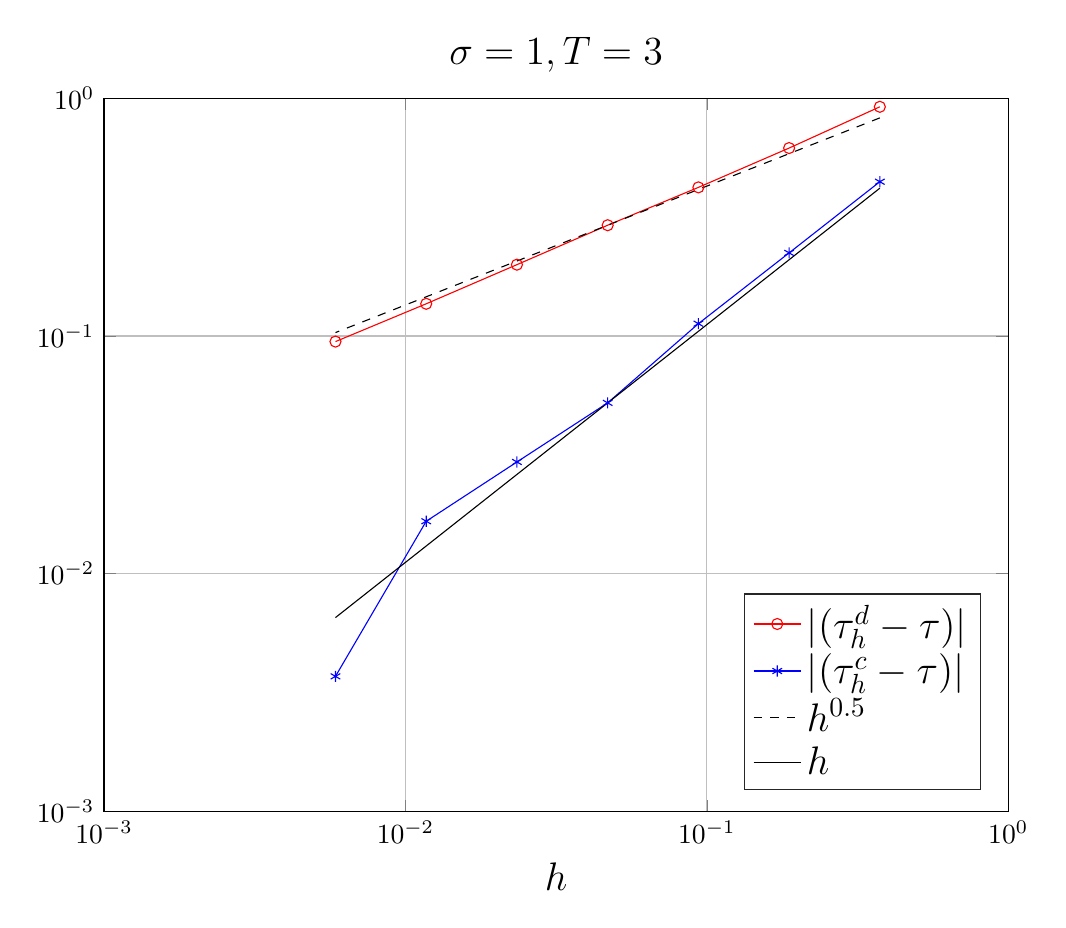
\begin{tikzpicture}

\begin{axis}[%
width=4.521in,
height=3.566in,
at={(0.758in,0.481in)},
scale only axis,
title={$\sigma = 1, T = 3$},
title style = {font=\Large},
xmode=log,
xmin=0.001,
xmax=1,
xminorticks=false,
xlabel={$h$},
xlabel style={font=\Large},
xmajorgrids,
ymode=log,
ymin=0.001,
ymax=1,
yminorticks=false,
ymajorgrids,
axis background/.style={fill=white},
legend pos = south east,
legend style={legend cell align=left,align=left,draw=white!15!black,font=\Large}
]
\addplot [color=red,solid,mark=o,mark options={solid}]
  table[row sep=crcr]{%
0.375	0.920558951920583\\
0.1875	0.617333951920583\\
0.09375	0.421846451920583\\
0.046875	0.292363639420583\\
0.0234375	0.199588639420583\\
0.01171875	0.136614420670583\\
0.005859375	0.0947198894205827\\
};
\addlegendentry{$|\E(\tau_h^d - \tau)|$};

\addplot [color=blue,solid,mark=asterisk,mark options={solid}]
  table[row sep=crcr]{%
0.375	0.445546451920583\\
0.1875	0.223658951920583\\
0.09375	0.112677701920583\\
0.046875	0.0523214519205826\\
0.0234375	0.0295214519205826\\
0.01171875	0.0166261394205827\\
0.005859375	0.00370153004558271\\
};
\addlegendentry{$|\E(\tau_h^c - \tau)|$};

\addplot [color=black,dashed]
  table[row sep=crcr]{%
0.375	0.82692924802669\\
0.1875	0.584727278841165\\
0.09375	0.413464624013345\\
0.046875	0.292363639420583\\
0.0234375	0.206732312006673\\
0.01171875	0.146181819710291\\
0.005859375	0.103366156003336\\
};
\addlegendentry{$h^{0.5}$};

\addplot [color=black,solid]
  table[row sep=crcr]{%
0.375	0.418571615364661\\
0.1875	0.20928580768233\\
0.09375	0.104642903841165\\
0.046875	0.0523214519205826\\
0.0234375	0.0261607259602913\\
0.01171875	0.0130803629801456\\
0.005859375	0.00654018149007282\\
};
\addlegendentry{$h$};

\end{axis}
\end{tikzpicture}%
 }  
        \caption{Approximation of $\tau$}
        \label{fig:KillOneDPhi}
    \end{subfigure}
    \begin{subfigure}{0.49\linewidth}
        \centering
        \resizebox{1\linewidth}{!}{% This file was created by matlab2tikz.
%
%The latest updates can be retrieved from
%  http://www.mathworks.com/matlabcentral/fileexchange/22022-matlab2tikz-matlab2tikz
%where you can also make suggestions and rate matlab2tikz.
%
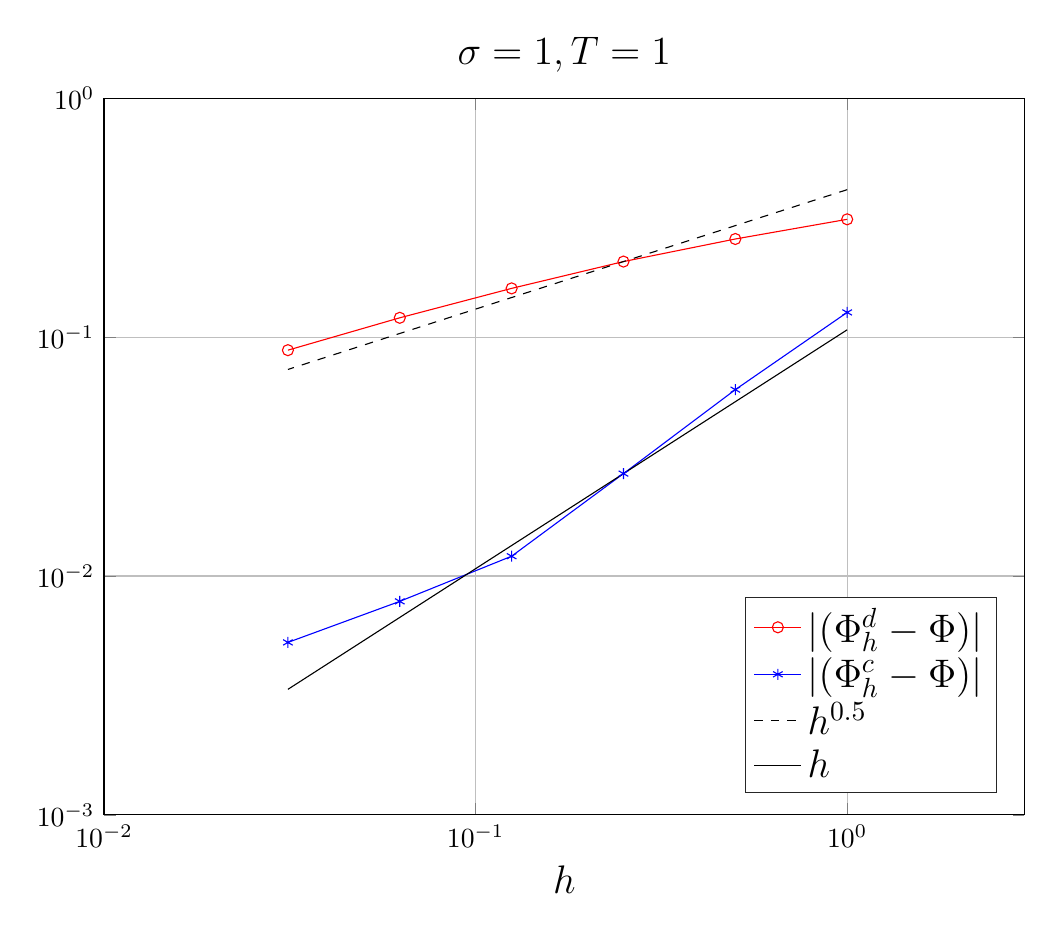
\begin{tikzpicture}

\begin{axis}[%
width=4.602in,
height=3.583in,
at={(0.772in,0.484in)},
scale only axis,
title={$\sigma = 1, T = 1$},
title style = {font=\Large},
xmode=log,
xmin=0.01,
xmax=3,
xminorticks=false,
xlabel={$h$},
xlabel style={font=\Large},
xmajorgrids,
ymode=log,
ymin=0.001,
ymax=1,
yminorticks=false,
ymajorgrids,
axis background/.style={fill=white},
legend pos = south east,
legend style={legend cell align=left,align=left,draw=white!15!black,font=\Large}
]
\addplot [color=red,solid,mark=o,mark options={solid}]
  table[row sep=crcr]{%
1	0.31134162505938\\
0.5	0.25753162505938\\
0.25	0.20716162505938\\
0.125	0.15999162505938\\
0.0625	0.12047162505938\\
0.03125	0.0881916250593803\\
};
\addlegendentry{$|\E(\Phi_h^d - \Phi)|$};

\addplot [color=blue,solid,mark=asterisk,mark options={solid}]
  table[row sep=crcr]{%
1	0.12689162505938\\
0.5	0.0602816250593803\\
0.25	0.0268316250593803\\
0.125	0.0121016250593803\\
0.0625	0.00783162505938029\\
0.03125	0.00527162505938028\\
};
\addlegendentry{$|\E(\Phi_h^c - \Phi)|$};

\addplot [color=black,dashed]
  table[row sep=crcr]{%
1	0.41432325011876\\
0.5	0.292970779762226\\
0.25	0.20716162505938\\
0.125	0.146485389881113\\
0.0625	0.10358081252969\\
0.03125	0.0732426949405564\\
};
\addlegendentry{$h^{0.5}$};

\addplot [color=black,solid]
  table[row sep=crcr]{%
1	0.107326500237521\\
0.5	0.0536632501187606\\
0.25	0.0268316250593803\\
0.125	0.0134158125296902\\
0.0625	0.00670790626484508\\
0.03125	0.00335395313242254\\
};
\addlegendentry{$h$};

\end{axis}
\end{tikzpicture}%
 }  
        \caption{Approximation of $\Phi$}
        \label{fig:ReflectOneDPhi}
    \end{subfigure}    
    \caption{Results for the two-dimensional case.}
\end{figure}
\end{frame}


